\documentclass[aspectratio=169,11pt]{beamer}
\newcommand{\footerlabel}{DEMO102 Networks \textbullet{} Lecture 1}
% 共用样式 —— 虚构示例课件（DEMO），内容全部自编，不来自任何真实课程。
% 用法：每份 deck 先 \documentclass，再定义 \footerlabel，最后 % 共用样式 —— 虚构示例课件（DEMO），内容全部自编，不来自任何真实课程。
% 用法：每份 deck 先 \documentclass，再定义 \footerlabel，最后 % 共用样式 —— 虚构示例课件（DEMO），内容全部自编，不来自任何真实课程。
% 用法：每份 deck 先 \documentclass，再定义 \footerlabel，最后 \input{_style}。
\usepackage[T1]{fontenc}
\usepackage{lmodern}
\usepackage{amsmath,amssymb}
\usetheme{default}
\setbeamertemplate{navigation symbols}{}
\setbeamercolor{frametitle}{fg=blue!50!black}
\setbeamerfont{frametitle}{series=\bfseries,size=\Large}
\setbeamercolor{title}{fg=blue!50!black}
\setbeamercolor{footline}{fg=black!60}
\setbeamertemplate{footline}{%
  \leavevmode\hbox{%
    \begin{beamercolorbox}[wd=.85\paperwidth,ht=2.5ex,dp=1ex,left,leftskip=1em]{footline}\footnotesize\footerlabel\end{beamercolorbox}%
    \begin{beamercolorbox}[wd=.15\paperwidth,ht=2.5ex,dp=1ex,right,rightskip=1em]{footline}\footnotesize\insertframenumber\end{beamercolorbox}}%
  \vskip0pt}
\setbeamertemplate{itemize items}[circle]
。
\usepackage[T1]{fontenc}
\usepackage{lmodern}
\usepackage{amsmath,amssymb}
\usetheme{default}
\setbeamertemplate{navigation symbols}{}
\setbeamercolor{frametitle}{fg=blue!50!black}
\setbeamerfont{frametitle}{series=\bfseries,size=\Large}
\setbeamercolor{title}{fg=blue!50!black}
\setbeamercolor{footline}{fg=black!60}
\setbeamertemplate{footline}{%
  \leavevmode\hbox{%
    \begin{beamercolorbox}[wd=.85\paperwidth,ht=2.5ex,dp=1ex,left,leftskip=1em]{footline}\footnotesize\footerlabel\end{beamercolorbox}%
    \begin{beamercolorbox}[wd=.15\paperwidth,ht=2.5ex,dp=1ex,right,rightskip=1em]{footline}\footnotesize\insertframenumber\end{beamercolorbox}}%
  \vskip0pt}
\setbeamertemplate{itemize items}[circle]
。
\usepackage[T1]{fontenc}
\usepackage{lmodern}
\usepackage{amsmath,amssymb}
\usetheme{default}
\setbeamertemplate{navigation symbols}{}
\setbeamercolor{frametitle}{fg=blue!50!black}
\setbeamerfont{frametitle}{series=\bfseries,size=\Large}
\setbeamercolor{title}{fg=blue!50!black}
\setbeamercolor{footline}{fg=black!60}
\setbeamertemplate{footline}{%
  \leavevmode\hbox{%
    \begin{beamercolorbox}[wd=.85\paperwidth,ht=2.5ex,dp=1ex,left,leftskip=1em]{footline}\footnotesize\footerlabel\end{beamercolorbox}%
    \begin{beamercolorbox}[wd=.15\paperwidth,ht=2.5ex,dp=1ex,right,rightskip=1em]{footline}\footnotesize\insertframenumber\end{beamercolorbox}}%
  \vskip0pt}
\setbeamertemplate{itemize items}[circle]

\usepackage{tikz}
\title{Computer Networks}
\subtitle{Lecture 1: Layering and Protocols}
\author{Demo Lecturer}
\date{Semester 2, 2026}

\begin{document}

\begin{frame}
  \titlepage
\end{frame}

\begin{frame}{What Is a Network?}
  \begin{itemize}
    \item \textbf{Hosts} (end systems) run applications
    \item \textbf{Links} carry bits between nodes (copper, fibre, radio)
    \item \textbf{Switches and routers} forward data towards its destination
  \end{itemize}
  \bigskip
  The hard part is not any single piece; it is making millions of independently
  built pieces work together.
\end{frame}

\begin{frame}{Why Layers? A Postal Analogy}
  Sending a letter abroad: you write it, the post office sorts it, a plane carries it.
  \medskip
  \begin{itemize}
    \item You do not know which plane is used -- and you should not need to
    \item Each step offers a \textbf{service} to the step above and uses the one below
    \item Any step can be replaced (a train instead of a plane) without changing the others
  \end{itemize}
  \medskip
  Layering = the same idea applied to network software.
\end{frame}

\begin{frame}{The Five-Layer Model}
  \begin{center}\small
  \begin{tabular}{llll}
    \hline
    Layer & Job & Example protocol & Unit of data \\
    \hline
    Application & what the user program says & HTTP, DNS & message \\
    Transport & process-to-process delivery & TCP, UDP & segment \\
    Network & host-to-host delivery across networks & IP & packet \\
    Link & delivery over one hop & Ethernet, Wi-Fi & frame \\
    Physical & bits on the medium & copper, fibre, radio & bit \\
    \hline
  \end{tabular}
  \end{center}
\end{frame}

\begin{frame}{Encapsulation}
  Each layer wraps the data from above with its own \textbf{header}.
  \bigskip
  \begin{center}
  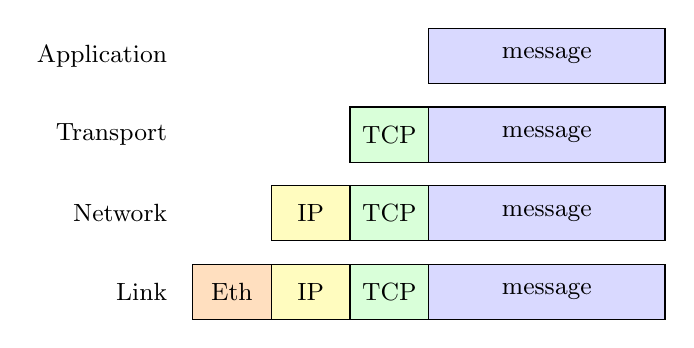
\begin{tikzpicture}[x=1cm,y=1cm,font=\small]
    \draw[fill=blue!15] (4,3) rectangle (7,3.7) node[midway]{message};
    \draw[fill=green!15] (3,2) rectangle (4,2.7) node[midway]{TCP};
    \draw[fill=blue!15] (4,2) rectangle (7,2.7) node[midway]{message};
    \draw[fill=yellow!25] (2,1) rectangle (3,1.7) node[midway]{IP};
    \draw[fill=green!15] (3,1) rectangle (4,1.7) node[midway]{TCP};
    \draw[fill=blue!15] (4,1) rectangle (7,1.7) node[midway]{message};
    \draw[fill=orange!25] (1,0) rectangle (2,0.7) node[midway]{Eth};
    \draw[fill=yellow!25] (2,0) rectangle (3,0.7) node[midway]{IP};
    \draw[fill=green!15] (3,0) rectangle (4,0.7) node[midway]{TCP};
    \draw[fill=blue!15] (4,0) rectangle (7,0.7) node[midway]{message};
    \node[anchor=east] at (0.8,3.35) {Application};
    \node[anchor=east] at (0.8,2.35) {Transport};
    \node[anchor=east] at (0.8,1.35) {Network};
    \node[anchor=east] at (0.8,0.35) {Link};
  \end{tikzpicture}
  \end{center}
\end{frame}

\begin{frame}{Protocol, Service, Interface}
  \begin{center}
  \begin{tabular}{lp{0.62\textwidth}}
    \hline
    Term & Meaning \\
    \hline
    Service & what a layer \emph{offers} to the layer above \\
    Interface & how the layer above asks for that service \\
    Protocol & the rules two \emph{peer} layers on different machines follow to talk \\
    \hline
  \end{tabular}
  \end{center}
  \medskip
  Changing a protocol inside one layer should not break the layers around it.
\end{frame}

\begin{frame}{Summary and Next Time}
  \begin{itemize}
    \item Layers hide detail: each offers a service upward and uses the service below
    \item Data is wrapped by one header per layer on the way down (encapsulation)
    \item Next lecture: the \textbf{physical layer} -- how bits actually travel, and the limits on how fast
  \end{itemize}
\end{frame}

\end{document}
